\documentclass[lettersize,journal]{IEEEtran}
\usepackage{amsmath,amsfonts}
\usepackage{algorithmic}
\usepackage{algorithm}
\usepackage{array}
\usepackage[caption=false,font=normalsize,labelfont=sf,textfont=sf]{subfig}
\usepackage{textcomp}
\usepackage{stfloats}
\usepackage{url}
\usepackage{verbatim}
\usepackage{graphicx}
\usepackage{cite}
\hyphenation{op-tical net-works semi-conduc-tor IEEE-Xplore}
% updated with editorial comments 8/9/2021

\begin{document}

\title{Evolutionary Multiobjective Surrogate-Assisted Neural Architecture for Intrusion Detection of Vehicle CAN Messages}

\author{Bin Cao, Tian Shan, IEEE Publication Technology,~\IEEEmembership{Staff,~IEEE,}
        % <-this % stops a space
\thanks{This paper was produced by the IEEE Publication Technology Group. They are in Piscataway, NJ.}% <-this % stops a space
\thanks{Manuscript received April 19, 2021; revised August 16, 2021.}}

% The paper headers
\markboth{Journal of \LaTeX\ Class Files,~Vol.~14, No.~8, August~2021}%
{Shell \MakeLowercase{\textit{et al.}}: A Sample Article Using IEEEtran.cls for IEEE Journals}

% \IEEEpubid{0000--0000/00\$00.00~\copyright~2021 IEEE}
% Remember, if you use this you must call \IEEEpubidadjcol in the second
% column for its text to clear the IEEEpubid mark.

\maketitle

\begin{abstract}
More and more electronic devices have emerged in the vehicle. It is very necessary to ensure the safety and reliability of the communication between the various electronic modules for drivers’ safety. Especially as the most commonly used communication protocol on vehicles, Controller Area Network (CAN) messages, has no security verification mechanism, which poses a great threat to the communication security on the vehicle. Neural architecture search (NAS) is a promising method for automatically design neural architectures. NAS adopts a search strategy to explore the predefined search space to find outstanding performance architecture with the minimum searching costs. In this paper we propose an intrusion detection model based deep neural network which is optimized by Multi-Objective Evolutionary Algorithm (MOEA) to promote accuracy and decrease complicity of the neural network. Through graph neural network(GNN) and convolutional neural network(CNN) to explore the internal logical feature and spatial feature of CAN. Because the different CAN length of the different functions of the vehicle CAN messages, we take advantage of reinforcement learning to dynamic get a CAN package which as a sample sent to our model. we also propose a method to converting original CAN to graph data by use of its time sequence feature. The CNN and GNN of the detection model are optimized by MOEA. CNN inherits the weight of parent, and GNN inherits the weight of supernet in the evolution process. Weight sharing shortens the time of individual adaptability evaluation. We performed an experimental study using the dataset collected from  the real world to evaluate our intrusion detection model. After the network evolution, the GNN flops decreased to 40\% of the supernet, but the intrusion detection accuracy reaches more than 95\%. The accuracy of convolution network was also improved by 5\% compared with the best individual of first generation. The accuracy of intrusion detection by combining the two models is more than 99\%.
\end{abstract}

\begin{IEEEkeywords}
Intrusion Detection of Controller Area Network (CAN), Multi-Objective Evolutionary Algorithm (MOEA), graph neural network (GNN), convolutional neural network (CNN)
\end{IEEEkeywords}

\section{Introduction}
\IEEEPARstart{I}{n} the last few decades, the implementation of automotive electronics has experienced a rapid growth \cite{1}. This trend has resulted in several changes in the vehicular ecosystem. Drive-by wire (DBW) technology, for example, uses of electronic or electrical systems in the control systems, such as the throttle, brake, and steering, which were traditionally controlled using mechanical linkages. CAN provides a simple and reliable communication protocol as the standard of an in-vehicle network \cite{2}, connecting not only sensors and controllers but also the Internet. The adoption of CAN accelerates the applications with the emergence of Vehicle-to-Vehicle (V2V) and Vehicle-to-Infrastructure (V2I) communication interfaces \cite{3}. However, the openness of the vehicular system increases the risk of malicious cyberattacks that can severely threat human life. However, the conventional in-vehicle networks are tremendously vulnerable with the cyberattacks as CAN is developed for an isolated physical system before. For example, every ECU sharing a CAN bus can obtain any ECU-to-ECU message. Furthermore, a CAN packet has no sender’s identification as shown in figure \ref{fig_1}. Koscher et al. \cite{4} conduct several experiments where a CAN message can be readily fuzzed by a packet injection and modification. Various attack scenarios e.g. disabling brakes and displaying wrong information on an instrument panel are shown in \cite{5, 6}. Attacks on the CAN bus can manifest in several ways. Diagnostic commands deployed during driving can cause malicious effects, e.g. locking the brakes to immobilize the car. However diagnostic commands should never be seen during normal driving, and so they are detectable trivially. Recent research works point the weakness of the security. 

\begin{figure}[!t]
\centering
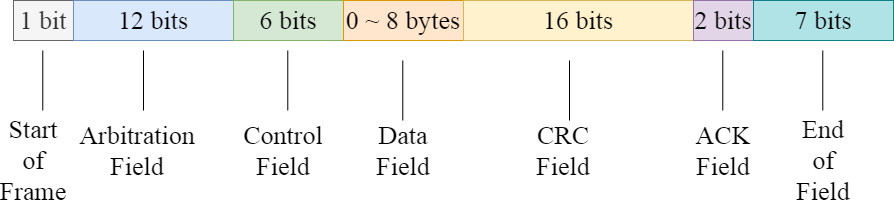
\includegraphics[width=3in]{CAN}
\caption{Format of the CAN data frame.}
\label{fig_1}
\end{figure}

Graph data are everywhere in fields \cite{7,8}, which is mainly used to process Non Euclidean data features, including social network field \cite{9}, text network field \cite{10} and biological network field \cite{11}. Graph neural network (GNN) is proposed to operate graph directly and solve graph related problem fields in an end-to-end manner \cite{12}. Relational modeling is crucial for many network or graphical data mining tasks, such as link prediction. GNN has recently been successfully applied in the real world, such as image recognition field \cite{13}, new drug discovery field \cite{14} and flow prediction field \cite{15}. In this work, the graph data are constructed by the time sequence characteristics of CAN, and the logical characteristics of CAN are extracted by the graph neural network. In reality, there are more dynamic graphs, and most of the work is to deal with dynamic graphs, such as social networks or financial networks. This dynamic graph changes the nodes of previous graph data or the connection between nodes as time goes by. This graph network uses RNN fields \cite{16,17} to learn the temporal characteristics of dynamic graphs, and spatiotemporal graph neural network architecture to learn the spatial characteristics of dynamic graphs \cite{18}. However, some graph data may be completely different at different times. Our work constructs the graph data of CAN, the nodes or connections of graph data constructed in the two time periods may be completely different. There is very little work to identify the graph network of such graph data. This model uses graph collapse network \cite{19} to detect such graph data.

Developing a custom learning architecture consisting of multiple GNN layers for specific scenarios (e.g., biological and physical network data) is still difficult, even for neural network experts. Falkner et al. \cite{20} pointed out that the deep learning algorithm is very sensitive to many hyperparameters. The work in literature field \cite{21} shows that the hyperparametric optimization (HPO) of GNNS is very important to achieve satisfactory results in practice. Therefore, the study of effective HPO methods for GNN is of great value for GNN to be applied to various practical problems. In order to automate the model selection process, neural architecture search (NAS) is widely used in fields \cite{22,23}, and has become the focus of deep learning research in recent years. NAS aims to explore the optimal combination of architecture components from the search space to maximize the model performance applicable to the target problem. So far, people have made great efforts to search convolutional neural network (CNN) architecture, which has promoted the latest progress of many important benchmark tasks, such as image classification fields on cifar10/100 and Imagenet \cite{24, 25}. In contrast, little work has been done on GNN learning of graphic structure data \cite{26,27,28}. NAS literature has proposed two main types of methods as the most effective problem-solving methods: reinforcement learning (RL) and evolutionary algorithm (EAS) \cite{28}. So far, the second technology has been ignored in the GNNs environment. The results show that both RL and EA can find equivalent models in terms of accuracy, and EA is faster in some cases. Two recent related work fields \cite{28,30} mainly focus on NAS based on reinforcement learning, and use recurrent neural network (RNN) as the controller to generate variable length strings describing GNN architecture to maximize the expected accuracy of the generated network architecture on the verification dataset. Although encouraging results have been achieved, the existing work has always faced the challenge of the following two shortcomings: hyperparametric invariance and high computational intensity. In addition, the controller usually generates candidate GNN architectures and evaluates them in a sequential manner, which is difficult to expand to a large search space.

NAS tasks can usually be described as a complex optimization problem \cite{29,31}. Generally speaking, the neural network with higher complexity can have higher recognition accuracy, but it will greatly increase the detection time of intrusion CAN messages. Our algorithm uses two conflicting objectives, namely, the accuracy of intrusion detection and the complexity of the model, for multiobjective optimization. In the field of computational intelligence, evolutionary algorithms (EAS) have been widely used to solve various neural network training problem fields \cite{32}, such as weight training field \cite{32}, architecture design field \cite{33} and learning rule adaptive field \cite{34}. Recently, evolutionary neural architecture search using EA as NAS optimizer has attracted more and more attention \cite{35,36,37}. The GNN gene field \cite{26} is proposed through the evolutionary method. It identifies the GNN architecture and trains the hyperparameters in two search spaces, and alternately optimizes the structure and hyperparameters of the graph network (such as learning rate and dropout). Our work puts them into one search space for search. The recognition rate of the graph network architecture found is more than 95\%, and the recognition rate of the graph network and convolution network combined is more than 99\%.

Neural network architecture search is a process, which generates and evaluates the hyperparameter settings iteratively until the preset stop conditions are met, so as to obtain the best solution. Usually, the objective function of neural network is selected as the fitness function to evaluate the hyperparameters. However, evaluation is usually very expensive because training GNN models requires a lot of computing resources. On the other hand, with the development of deep learning, neural network has more and more layers or various other optional hyperparameters (such as activation function and optimization method), which leads to a large search space and increases the difficulty of search. With the increase of network components, the consumption of computing resources for searching the network is huge, and tedious and arduous efforts are made for GNN architecture adjustment and optimization. Therefore, the existing neural architecture search work is based on how to find the best solution with less experiments, reduce the evaluation cost and improve the exploration ability. Although EAS has competitive search performance in various optimization tasks\cite{38}, as a group based optimization method, its calculation cost is usually high. This is especially true for EvoNAS, because EAs usually requires a large number of fitness assessments, and each fitness assessment in NAS is computationally expensive, because it usually involves training deep neural networks from scratch on a large amount of data. For example, AE-CNN requires 27 GPUs to obtain an optimized CNN architecture on the cifar10 dataset. Some works search the hyperparameters of graph networks, and save computing resources by quickly evaluating individuals. For example, \cite{39} proposes parallel graph architecture search to improve search efficiency. In our work, when convolution networks evolve, offspring inherit the weights of parent networks and graph neural networks inherit the weight parameters of hypernetworks to achieve rapid individual adaptability evaluation.

Deep reinforcement learning is the combination of reinforcement learning and deep learning. This research field can solve a series of complex decision-making tasks that could not be completed by machines before. Therefore, deep RL has opened up many new application fields in medical care, robotics, smart grid, finance and other fields \cite{40}. The length and content of the CAN messages are different when the vehicle performs different functions. Based on this inspiration, we use reinforcement learning to obtain the length of the CAN messages for each intrusion detection. The experimental results show that the intrusion detection rate of the model increases by 5\% after using the variable length CAN compared with random length. The reinforcement learning network learns the feature vector of the graph convolution output in each graph network as each state input to the reinforcement learning actor network, and the reinforcement learning outputs the next action, that is, the length of the next CAN message. In the early reinforcement learning, there was an overestimation of the real action value \cite{41}, and \cite{42} established two value networks to solve the overestimation problem. Reinforcement learning can be divided into discrete type and continuous type according to the types of output actions. The meaning of action in the model is the length of the output CAN messages. We give the range of message length. The integer value between the minimum and maximum length can be taken. Based on the above requirements, we use TD3\cite{43} network as a neural network to dynamically obtain the length of CAN messages which are sent to intrusion detection model everytimes.

To address the aforementioned challenges, In this paper, we propose a deep neural network intrusion detection model based on evolutionary multiobjective surrogate-assisted neural architecture search to detect CAN intrusion, such as denial-of-service (DoS) and spoofing attacks, with significantly high accuracy and low complicity. In summary, the main contributions of this paper are as follows:

\begin{itemize}
\item{A multiobjective evolutionary GNN detection model is proposed, which takes the detection accuracy and the model flops as the optimization objectives. In the evolution process, the node inheritance strategy is adopted to shorten the time of individual evaluation.}
\item{A method of converting CAN message into graph data is proposed. Two connected nodes of graph data are constructed according to the timing information of two adjacent timestamps. The logic features in CAN are extracted, so that CAN messages can be classified by GNN.}
\item{A model combining GNN and CNN is proposed to detect CAN intrusion messages, and reinforcement learning network is used to dynamically collect intrusion detection samples of CAN. During the training of detection model, the logic and spatial characteristics of CAN are learned at the same time.}
\end{itemize}

The rest of this paper is organized as follows. Section \ref{section_related_work}  introduces the related work of our proposed model. Section \label{section_architecture_search_space} describes the encoding of neural network architectures, followed by the details of the proposed intrusion detection model and the method of converting to graph data from CAN in Section \ref{section_proposed} . Experimental settings and results are presented in Section \ref{section_result}, respectively. Finally, Section \ref{section_conclusion} concludes the paper and proposes some points can be improved of our model in the future.

\section{RELATED WORK}\label{section_related_work}
\subsection{Conventional intrusion detection of CAN}
The CAN frame is generally unable to support Message  Authentication Code (MAC) \cite{44} and other methods of securing communication. Some researchers have attempted to either create new protocols or spread MAC across multiple transmissions. in \cite{45}, Tashiro et al. for tampering detection can be conducted for both individual frames and entire sections, they propose a protocol that provides protection against replay, masquerading and injection attacks by sending a partial MAC in each frame. Nowdehi et al. \cite{46} examine many of these altered protocols in light of five criteria for potential CAN message authentication solutions from an industry perspective. They found that no solutions met all the criteria. VatiCAN takes the approach of utilizing maintenance support, “sufficient implementation details” and no excessive overhead, while WooAuth alters the extended CAN protocol to allow more space for authentication codes. Finally, the authors suggest that the CAN bus might “be fundamentally unsuited for secure communication”. \cite{46}

\subsection{Deep learning intrusion detection of CAN}
Intrusion detection strategy (IDS) can combine machine learning to train itself to identify abnormal behavior, which can be used as an alternative or supplement to MAC. IDS can prevent spoofing, injection, bus shutdown and denial of service attacks. In \cite{47}, Choi et al. Introduced a method called voltage IDS, which uses the inconsistency of ECU signals, first conducts training and testing, identifies the signal characteristics at this stage, and then uses the training data to verify whether the ECU has been damaged. Voltage IDS can detect camouflage attacks by using multi-class classifiers, one of which corresponds to an ECU. It predicts the most likely sender and compares this information with the actual can ID of the message. If they are different, a camouflage attack is detected. In \cite{48}, song et al, by converting the ID part of the CAN frame into binary. Used the changed ResNet model to extract the features of the binary text, and learned the features of the intrusion message and the normal message for intrusion detection. Their experimental results show that compared with the traditional machine learning algorithm, this algorithm has lower false positive rate and false positive rate. In \cite{49}, Taylor et al. Proposed using deep learning methods for intrusion detection, because they are generated directly from the bit stream on the network, the execution efficiency of these functions is high and the complexity is low. This technology monitors the exchange packets in the vehicle network while training the characteristics offline, and provides a real-time response to the attack with a significantly high detection rate in their experiment.

\subsection{Neural architecture search by EA}
neural architecture search (NAS) aims to automatically design network architecture, which is essentially an optimization problem of finding an architecture with the best performance in specific search space with constrained resources \cite{50, 51}. Sun et al. \cite{52} used EA with variable coding length to automatically evolve the architecture of CNN. William et al. \cite{53} introduced an evolutionary NAS coding strategy based on directed acyclic graphs (DAG), which has better performance than the randomly generated CNN architecture. Real et al. propose Amoebanet \cite{54}, which uses improved tournament selection to evolve network groups, and achieves better results on Imagenet than the handmade model. Wang et al. \cite{55} designed an effective evolutionary algorithm to optimize the generator within the framework of GANs. This method can effectively improve the generation performance and training stability of GAN model. Yin \cite{56} uses evolutionary multiobjective method to design CNN architecture, which uses probabilistic SMBO to maximize classification performance and minimize network reasoning time. Elsken et al. \cite{57} described NAS as a bi-objective optimization problem, in which two objectives are to maximize performance and minimize computing resources. Lu et al. \cite{58} proposed nsganet, which can automatically design the network, maximize the model performance and minimize floating point operations (flops). 

\subsection{Surrogate}
A major disadvantage of EvoNAS is that in the process of evolutionary optimization, each new candidate neural network needs to be trained on the training dataset and then evaluated on the validation dataset to avoid over-fitting. Therefore, if the network is large and the training dataset is large, the architecture evaluation in EvoNAS may take several hours. Because EAS is a kind of group based search methods, they usually need a lot of fitness evaluation, which makes EvoNAS computationally difficult to implement. For example, on CIFAR10 and CIFAR100 datasets, CNN-GA \cite{59} consumes 35 GPU days and 40 GPU days respectively, genetic CNN method \cite{60} consumes 17 GPU days, and large-scale evolutionary algorithm \cite{61} consumes 2750 GPU days. Therefore, in the case of limited computing resources, the agent model can accelerate the fitness evaluation in EvoNAS. Agents are divided into high-level agents and low-level agents. The high-level agent and low-level agent represent the architecture level and the parameter level in the architecture respectively. High level agent representation predicts the accuracy of different neural networks by parameterizing the neural network architecture. However, the low-level agent solves the complexity of using SGD optimization from scratch for each architecture after searching multiple architectures. The low-level agent is given a trained hypernetwork and neural network structure including all sub architectures. The weight of the neural network architecture inherits the weight from the hypernetwork. In the search process, the accuracy of using the weight inherited from the hypernetwork becomes the standard for selecting the architecture. However, the correlation between the accuracy of prediction architecture and the final accuracy of neural architecture through weight sharing is not close. The neural architecture reference MSuNAS \cite{62} we searched is not only sharing the weight of hypernetwork, but also fine-tuning through training again. MetaQNN \cite{63} uses the agent model to predict the final accuracy of candidate architectures (as time series prediction) from the first 25\% learning curve of SGD training. PNAs \cite{64} uses an alternative model to predict the accuracy of the network architecture, adding an additional branch to the unit structure, which is repeatedly stacked together. Both methods use the agent method to evaluate the performance of neural architecture. However, the correlation between the prediction accuracy of this method and the actual accuracy of the model is relatively low. OnceForAll \cite{65} also uses an agent model to predict the accuracy of architecture coding. However, the agent model is trained offline for the whole search space, so it needs a large number of samples to learn. ChamNet \cite{66} trains many architectures through complete low-level optimization, and selects only 300 high-precision samples with different efficiency (trigger, delay, energy) to train alternative models offline. Our model only conducts online learning on samples close to Pareto frontier, which significantly improves the efficiency of architecture search. Our model evaluation method draws lessons from the idea of MSuNAS.

\section{ARCHITECTURE SEARCH SPACE}\label{section_architecture_search_space}
This section introduces the search space of the model, including the search space of graph neural network and convolution network. The search of graph neural network includes structure and hyperparameter search. The structure search includes the number of layers of the graph convolution layer and the width of the prediction layer of the graph network. Hyperparameter search includes learning rate, activation function type, dropout rate, etc. Convolution network is a convolution network architecture \cite{48} that refers to the work of detecting CAN by convolution network. Its architecture is manually designed and consists of one stem part and four res convolution block parts. The convolution part of our model retains the stem part and extracts eight positions on the four convolution blocks. There are five options for each of these eight locations.

\subsection{GNN architecture search}
The specific genes and corresponding relationships are shown in Table~\ref{table1}.The chromosome is divided into nine parts. The first part of chromosome is position 0. There is a gene indicating whether to use the direction information of graph data constructed by CAN IDs. The graph data can determine the direction of the edge of the directed graph according to the sequential relationship between two adjacent frames. Specifically, the CAN IDs of the previous frame points to the next frame. Although using the direction of constructing graph data will make more use of the information of graph data, the experimental results show that using more graph information does not necessarily improve the recognition accuracy. See the next section for the analysis of specific experimental results. According to the formula in the previous section, it is necessary to obtain the Laplace matrix of each subgraph and calculate the eigenvector of each subgraph. Whether to use regularization for Laplacian matrix before calculating the eigenvector of each subgraph. The regularized Laplacian matrix $L_{norm}$ and the nonregularized Laplacian matrix $L$ of the graph network are expressed as \eqref{deqn_ex_7}\eqref{deqn_ex_8}. 

\begin{equation}
\label{deqn_ex_7}
L\ =\ D\ -\ A
\end{equation}

\begin{equation}
\label{deqn_ex_8}
L_{norm}\ =\ I\ -\ D^{-1/2}AD^{1/2}
\end{equation}

Where $A$ represents the adjacency matrix of graph data and $D$ represents the degree matrix of graph data.The third part of the chromosome, positions 2 to 3, is the depth of the two GCN blocks. One GCN block is laid before graph coarsen, and the one is laid after graph coarsen. The fourth part of chromosome, positions 4 to 5, is the number of neurons in each layer of the prediction layer.In the process of evolutionary algorithm search, the neural network architecture refers to \cite{62,67}, are dynamically changed.The appropriate number of layers of graph convolution and the number of neurons in the prediction layer can achieve good detection accuracy while the complexity is not high. Parts 5 to 7 of chromosome, positions 6 to 8, represent the hyperparameters in the network architecture, such as dropout rate, learning rate, etc. Chromosome Part 8, positions 9 to 10, respectively represent how to reduce the dimension into a one-dimensional vector after each convolution block outputs the convolution result. There are three options: sum, average and maximum for each dimension. Part 9 of chromosome represents the activation function after the end of convolution or fully connection layers. 

\begin{table*}[!t]
\caption{GNN search space\label{table1}}
\centering
\begin{tabular}{cccc}
\hline
Part & Position & Meaning	 & Search space\\
\hline
1 & 0 & directed/undirected graph & directed undirected\\
2 & 1 & Whether Normalization of subgraph & not normalization normalization\\
3 & 2-3 & Layers of GCN & one two three\\
4 & 4-5 & Proportion of neurons in prediction layer & 0.25 0.5 0.75 1.00\\
5 & 6	 & Dropout & 0.005 0.01 0.02 0.03 00.4 0.05\\
6 & 7 & Weight Decay Rate & 5e-4 8e-4 1e-3 4e-3\\
7 & 8	 & Learning Rate & 5e-4 1e-3 5e-3 1e-2\\
8 & 9-10 & way to merge the vectors of every GCN layer & sum average max\\
9 & 11-18 & Activation function & sigmoid tanh relu  leaky\_relu relu6\\
\hline
\end{tabular}
\end{table*}

\subsection{CNN architecture search}
Deep convolution networks, such as the variants of Inception and ResNet, are designed to build neural networks by stacking multiple blocks. The neural network architecture design includes the determination of depth (number of layers), width (number of channels) and spatial resolution change (number of pool layers), while the block structure design specifies hierarchical connection and local calculation. Through this block design method, the generated model can not only achieve high performance, but also be extended to different datasets and tasks.

An operation space is defined by a set of possible basic components of network architecture and known successful modules designed by human experts. The five operations used in this study and the corresponding genotype-phenotype mapping are shown in Table~\ref{table2}. In the table, spatial separable convolution (SP) and deepwise separable convolution (DW) can reduce network parameters without sacrificing network performance. Here, we use two DW operations and two SP operations, and the kernel size respectively is 3 × 3 and 5 × 5, referred to as SP3, DW3 and SP5, DW5.

\begin{table}[!t]
\caption{CNN search space\label{table2}}
\centering
\begin{tabular}{cccc}
\hline
Operation type & Kernel size & Short name & Code\\
\hline
Spatial Separable Convolutions	 & 3 & SP3 & 0\\
Spatial Separable Convolutions	 & 5 & SP5 & 1\\
Depthwise separable convolution & 3 & DW3 & 2\\
Depthwise separable convolution & 5 & DW5 & 3\\
Normal convolution & 3 & 3*3 & 4\\
\hline
\end{tabular}
\end{table}


\section{PROPOSED INTRUSION DETECTION MODEL}\label{section_proposed}
The architecture we proposed is shown in the figure and can be divided into two parts of requiring CAN part and intrusion detection part. Requiring CAN part is constructed by reinforcement learning (RL) network to dynamically collect CAN messages. Intrusion detection part is constructed by graph neural network (GNN) and convolutional neural network (CNN). The network architecture of GNN and CNN is optimized by EA. The parts optimized by EA are marked with dotted lines in the figure \ref{fig_2}. They are the convolution layer of CNN, the GCN layer of graph neural network and the full connection layer and etc. The specific search space and search process are described below. At the same time, using the advantages of two different neural networks, GNN has the advantage of extracting logical features and CNN has the advantage of extracting spatial features. Finally, the output results of the two networks are integrated to obtain the final result.

\begin{figure*}[!t]
\centering
{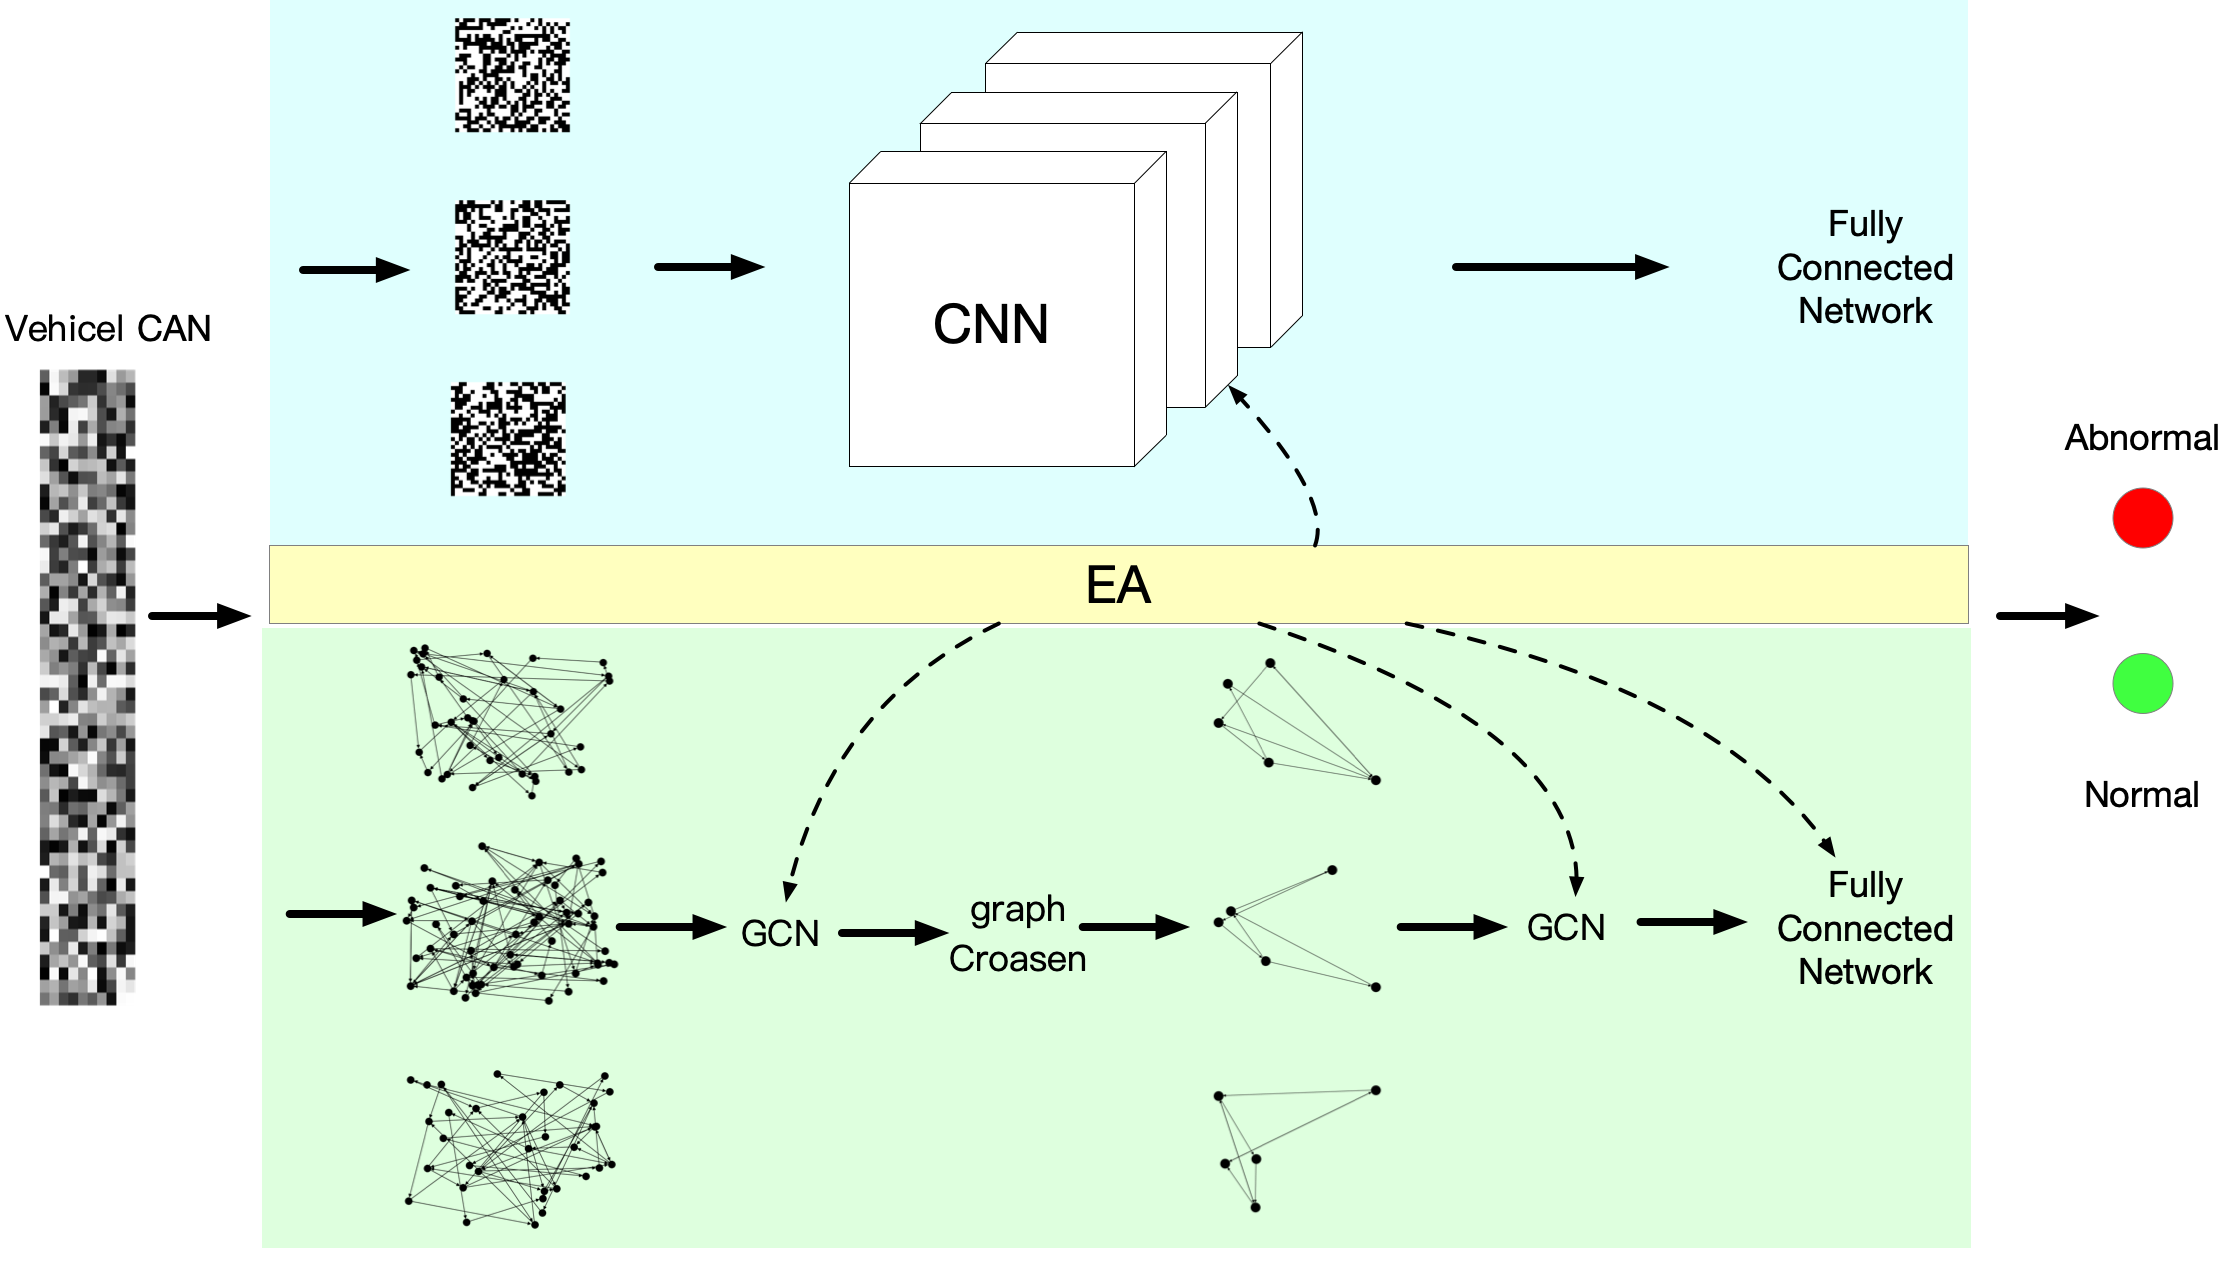
\includegraphics[width=7in]{evo-frame}%
\label{Overall framework of network architecture.}}
\hfil
\caption{Overall framework of network architecture.}
\label{fig_2}
\end{figure*}

\subsection{Collect CAN by Reinforcement Learning (RL)}
RL network is able to dynamic collect CAN messages of every detect sample which will send to GNN and CNN. Before each intrusion detection, a certain length of CAN messages is dynamically collected as a sample input to the detection network. In the vehicle can message, the message data of different functions or the message of the same function may also need different frames to complete, so the RL network is used to solve the problem of dynamic acquisition. Before training RL network, a GNN with intrusion detection ability is trained first. When training the GNN, the length of input is generated randomly. There are two convolution layers in our GNN. The output of the convolution layer is converted into one-dimensional vectors, and the two one-dimensional vectors are combined as the state input of RL network. The reward function is designed by using the recognition results of GNN. If the graph network recognition is correct, it will get a positive reward, and if the recognition is wrong, it will get a negative penalty. The RL network architecture design of this work refers to TD3\cite{43}. To avoid overestimation of value network, RL network is composed of two value networks and two action networks, and the output is discrete. The dimension of reinforcement learning network output is the difference between the maximum CAN length and the minimum CAN length of intrusion detection. As shown in \eqref{deqn_ex_1}.

\begin{equation}
\label{deqn_ex_1}
%x = \sum_{i=0}^{n} 2{i} Q.
\footnotesize {{output\_dim}_{RL}\ =\ MAX(CAN\_LEN)\ -\ MIN(CAN\_LEN)}
\end{equation}

\subsection{Intrusion detection by Graph Neural Network (GNN)}
First, we set the previous frame of message to point to the next frame of message. Because the message ID is limited, not all message will point to a new message, it may point to a message frame that has appeared before. The direction relationship of the converted graph data are related to the time sequence of the message frame sequence. A sequence of CAN IDs always indicates different functions in the vehicle, and whether the logic of the execution sequence of the functions is reasonable or not can be learned by the GNN. For example, a large acceleration signal appears when braking, or a vehicle ignition signal appears without a car key signal. These are unreasonable logic. It is very likely that an intrusion message has appeared on the CAN bus, which has practical significance. For the GNN to learn more abstract features, we input a partial graph of sequence data to determine whether the message is an intrusion message, instead of inputting one or two frames of message. Our proposed approach is shown in figure \ref{fig_3}.

\begin{figure*}[!t]
\centering
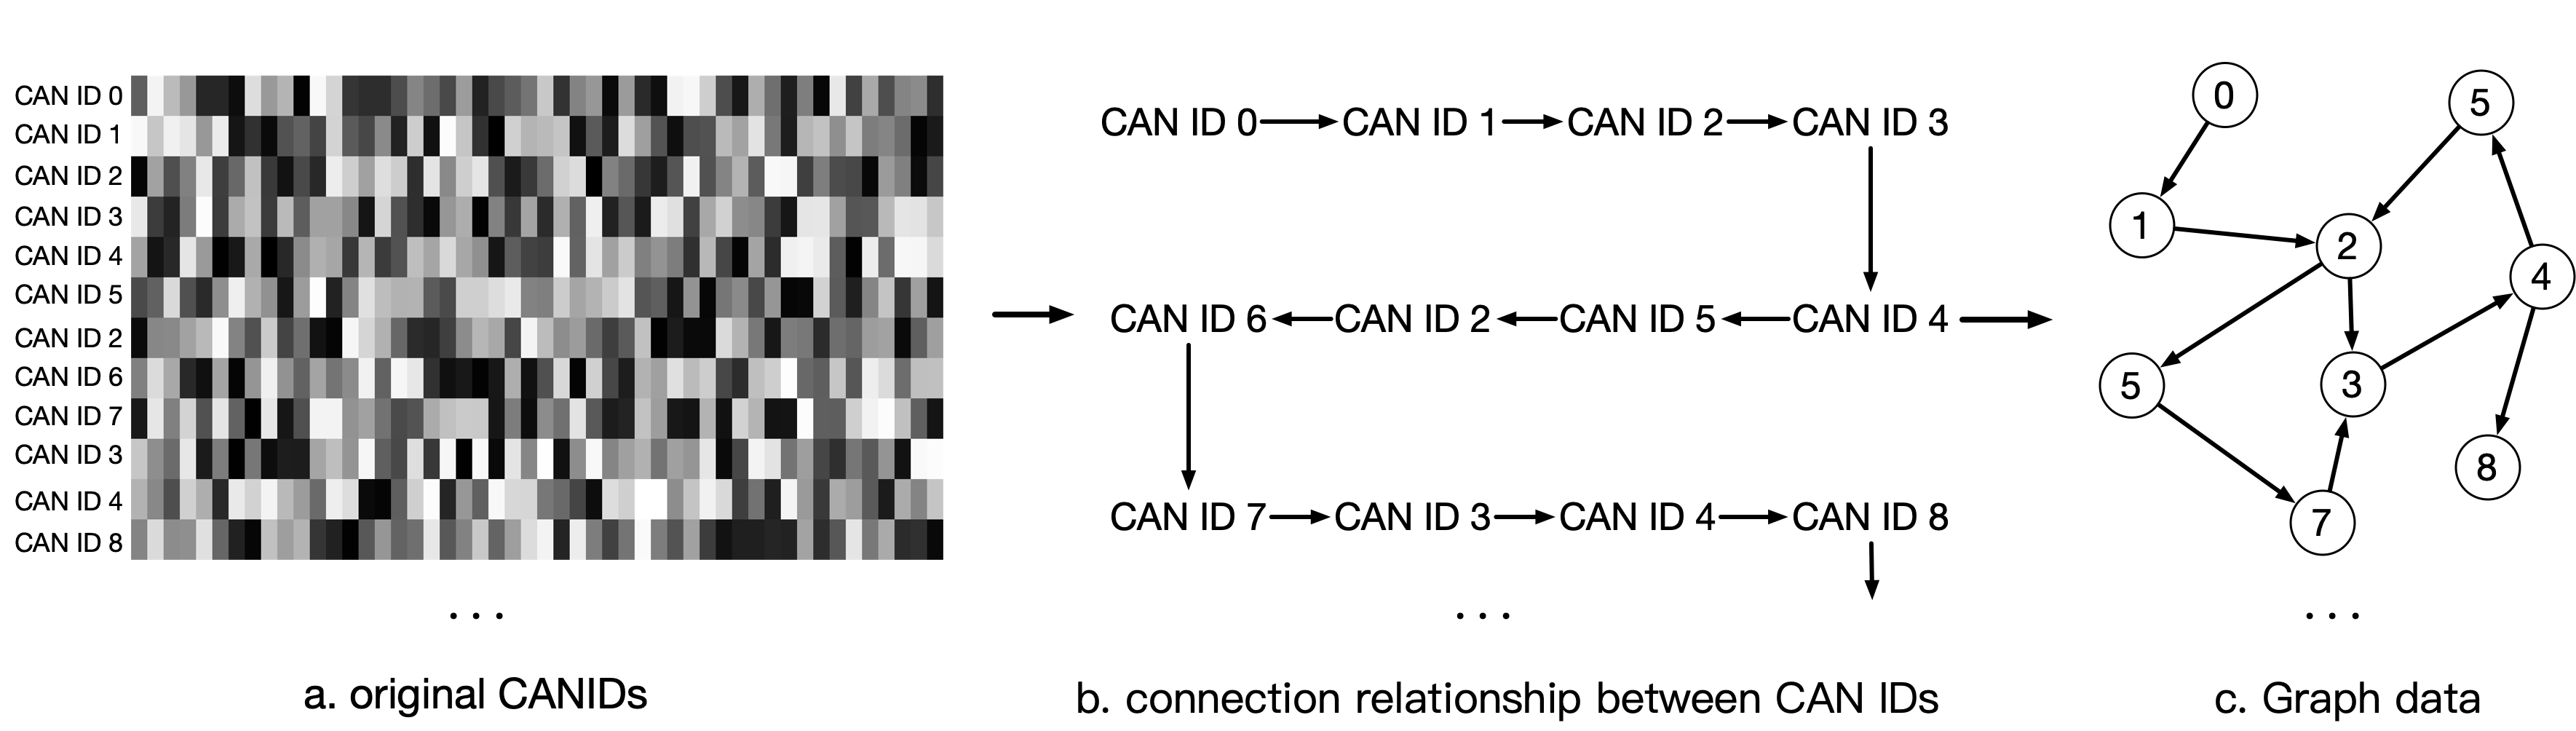
\includegraphics[width=7in]{graph-data}
\caption{Construct graph data from original CAN.}
\label{fig_3}
\end{figure*}

The graph neural network in this work is a graph level classification task, and the network architecture of graph classification task refers to \cite{19}. It is to divide the constructed graph data into several clusters by clustering method. Each cluster can be regarded as a subgraph of graph data to obtain the eigen matrix of a series of subgraphs. Using eigenvectors to construct the pooling matrix, each subgraph is pooled into a super node.  Graph G connected by given K subgraphs, C is a part of G. $N_k$ represents the number of nodes in the subgraph $G^{(k)}$. $\Gamma^{\left(k\right)}$ is the list of nodes in the subgraph $G^{(k)}$. Each subgraph can be regarded as a super node of graph G. Define sampling operator $C^{\left(k\right)}\in\mathbb{R}^{N\times N_k}$ as follow:

\begin{equation}
\label{deqn_ex_2}
C^{\left(k\right)}\left[i,j\right]=1\ if\ and\ only\ if\ \Gamma^{\left(k\right)}\left(j\right)=\upsilon_i
\end{equation}

$C^{\left(k\right)}\left[i,j\right]$ represents the element in i-th row and j-th column of $C^{\left(k\right)}$, $\Gamma^{\left(k\right)}\left(j\right)$ represents the jth node in the node list $\Gamma^{\left(k\right)}\left(j\right)$. This operation indicates the correspondence between the node in the subgraph $G^{(k)}$ and the original graph G. Because Fourier transform can convert the graph signal to the frequency domain and take the signal information and the structure information of graph data into account, we refer to \cite{19} and use Fourier transform to design pooling operation. The pooling operation pools the constructed graph signal G into $G_{coar}$. Pooling operation is based on the Fourier transform of each subgraph ${{G^k}}_{k=1}^K$. The Laplace matrix of the subgraph $G^{(k)}$ is $L^{(k)}$. $u_1^{(k)}, …, {\ u}_{N_k}^{(k)}$ represents the all eigenvectors of the Laplacian matrix $L^{(k)}$ of the k-th subgraph. Then use the upsampling operation $C^{(k)}$ to upsample the eigenvector to the whole graph G. The upsampling equation is represented by \eqref{deqn_ex_3}.

\begin{equation}
\label{deqn_ex_3}
{\bar{u}}_l^{(k)}=\mathbf{C}^{(k)}\mathbf{u}_l^{(k)},l=1\ldots N_k
\end{equation}

$\Theta_l\ \in\ \mathbb{R}^{N\times K}$ represents the pooling matrix containing the L-th eigenvector of all subgraphs.

\begin{equation}
\label{deqn_ex_4}
\mathrm{\Theta}_l=\left[{\bar{u}}_l^{\left(1\right)},\ldots,{\bar{u}}_l^{\left(k\right)}\right]
\end{equation}

Each subgraph does not necessarily have the same number of nodes, that is, the number of eigenvectors of each subgraph is not necessarily equal. $N_{max}\ =\ \underset{k\ =\ 1,...,K}\max{N_k}$ represents the maximum number of nodes in all subgraphs. For the subgraph $G^{(k)}$ owns $N_k$ nodes, the lst pooling operation is expressed as:

\begin{equation}
\label{deqn_ex_5}
X_l\ =\ \mathrm{\Theta}_l^TX
\end{equation}

$X_l$ indicates the result of the L-th pooling operation. The k-th row of $X_l$ contains the information of the k-th subgraph, that is, the k-th super node. Based on the above structure, we can construct $N_{max}$ times of pooling operation, and combine the results of all pooling operations to form the coarsen matrix.

\begin{equation}
\label{deqn_ex_6}
X_{coar}\ =\ [X_0,...,X_l,\ ..X_{N_{max}}]
\end{equation}

In some other graph classification tasks using pooling method, the sum or average method is used to treat each node in the subgraph indiscriminately, and the structure information of nodes in each subgraph cannot be extracted. In our work, we pool the graph data once, and do a graph convolution operation to extract features before and after pooling. Finally, the outputs of the two graph convolutions are transformed into one-dimensional vectors by summation or averaging, and the two one-dimensional vectors are spliced into one input to the full connection layer for classification. 

The crossover and mutation operations of the GNN are shown in the figure \ref{fig_4} and \ref{fig_5}. The crossover operation is to select two parents randomly in the population, and then randomly select the crossover point on each parent, and the separated parts are exchanged to generate two new offspring individuals. Mutation operation is to select a parent in the population with mutation probability, and then randomly select the mutation point on the parent to cause gene mutation.

\begin{figure*}[!t]
\centering
\includegraphics[width=7in]{gnn-cross}
\caption{GNN crossover operation.}
\label{fig_4}
\end{figure*}

\begin{figure*}[!t]
\centering
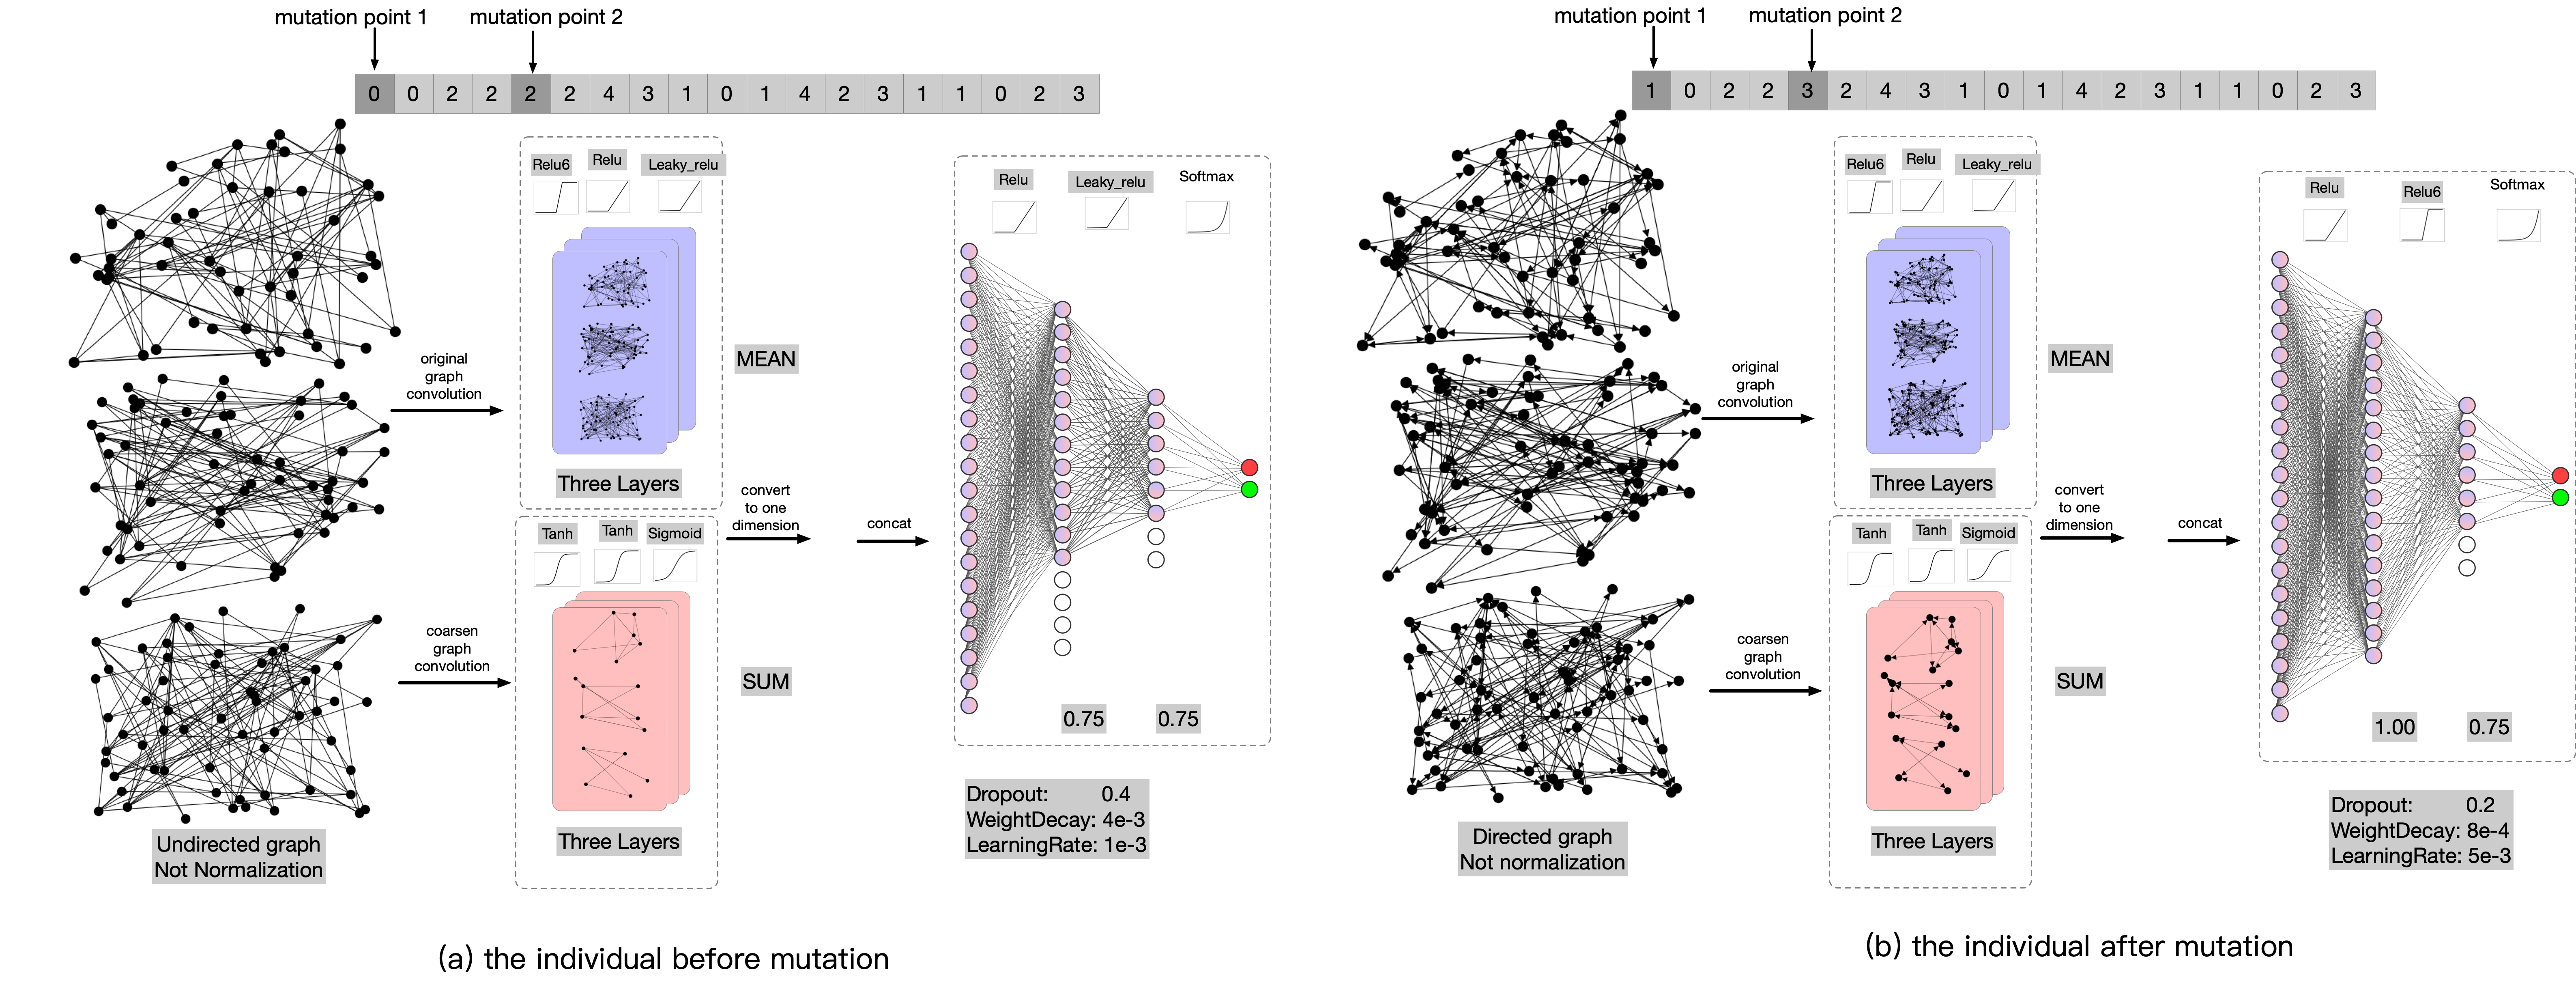
\includegraphics[width=7in]{gnn-mutation}
\caption{GNN mutation operation.}
\label{fig_5}
\end{figure*}

\subsection{Intrusion detection by convolutional neural network (CNN)}

In this paper, the hexadecimal CAN IDS is transformed into binary to form a sample similar to the image. Each pixel is 0 or 1 respectively. According to the reference paper, the number of ID bits of vehicle CAN extended frame is 29 bits, and 29 frames are collected to construct $29\times29$ samples.  We follow the same block level design method as in \cite{68,69,70}. Block is a small convolution network. To deal with different intermediate information more effectively in forward propagation, four kinds of convolution blocks, shown in figure \ref{fig_6}, are designed according to the different grid sizes of feature mapping. At the same time, the reduction block is designed to increase the deep receptive field, and halve the grid size of the feature map by applying all operations in steps of 2. According to the Convention of modern CNN Architecture \cite{71,72,73}, when the grid size of the feature graph is halved, we double the number of channels (filters) of the block to maintain a roughly constant hidden state dimension.

Inception ResNet is a kind of deep convolution model. It is designed to divide images into 1000 categories in the field of image classification, and shows very excellent performance. The overall architecture of the CNN is shown in Figure 5. The input size is 29$\times$29$\times$1, and the input data size is converted to 13$\times$13$\times$28 through the stem module. After the four modules optimized by EA, the data size is 2$\times$2$\times$896. Finally, the data are transformed into a binary classification vector with dimension 2 through the softmax module. The whole convolution network architecture is shown in figure \ref{fig_6}.

\begin{figure}[!t]
\centering
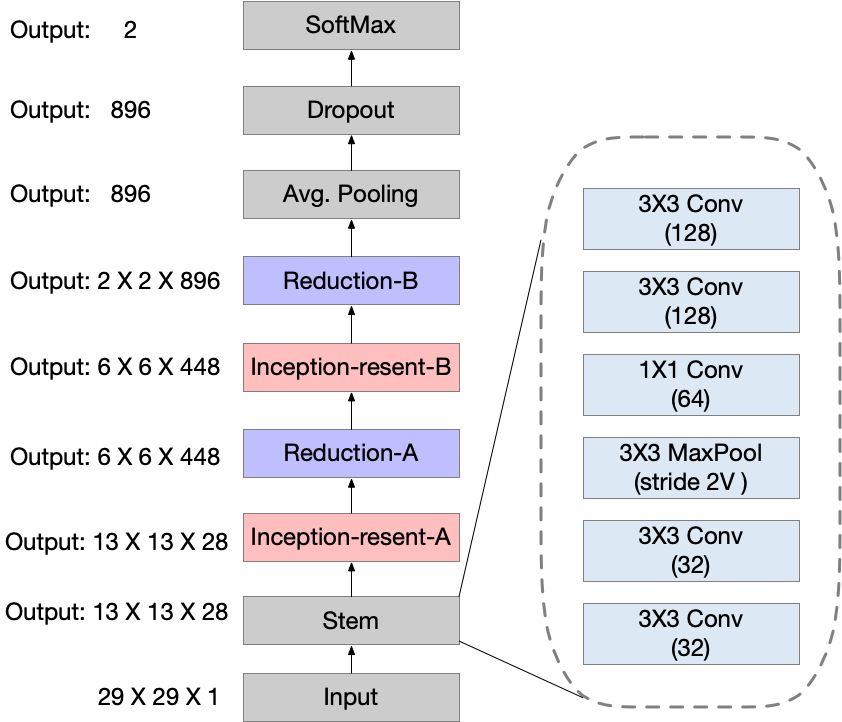
\includegraphics[width=3in]{cnn-overall}
\caption{Res-Inception blocks of CNN.}
\label{fig_6}
\end{figure}

Because the individual is retrained every time, the amount of calculation required is very huge. To improve the evaluation efficiency of genetic algorithm, agent method is used to exchange the weight parameters of corresponding neural network positions in the process of crossover operation and mutation operation. 
It can be seen from the schematic diagram of four different convolution blocks that the number of gene channels in each convolution block is different, and the number of gene channels in each convolution block is the same, which has no impact on the crossover operation, but will affect the mutation operation. At two gene exchange positions on a chromosome, and the corresponding weights of the neural network need to be exchanged, so the number of channels of the two genes needs to be the same. Both RedA and ResB convolution blocks have only one gene, and ResA and RedB convolution blocks have three genes respectively. Therefore, mutation can only be performed in ResA block or RedB block.
The crossover operation of evolution part first takes out two parent individuals by the tournament method of n=2, then randomly selects the intersection on each parent, disconnects at the intersection, and exchanges the separated parts to generate two new offspring individuals. The crossover process shown as figure \ref{fig_7}.  Mutation operation is to mutate each parent with mutation probability p, and then randomly select two points on the parent to exchange. The mutation process shown as figure \ref{fig_8}.

\begin{figure*}[!t]
\centering
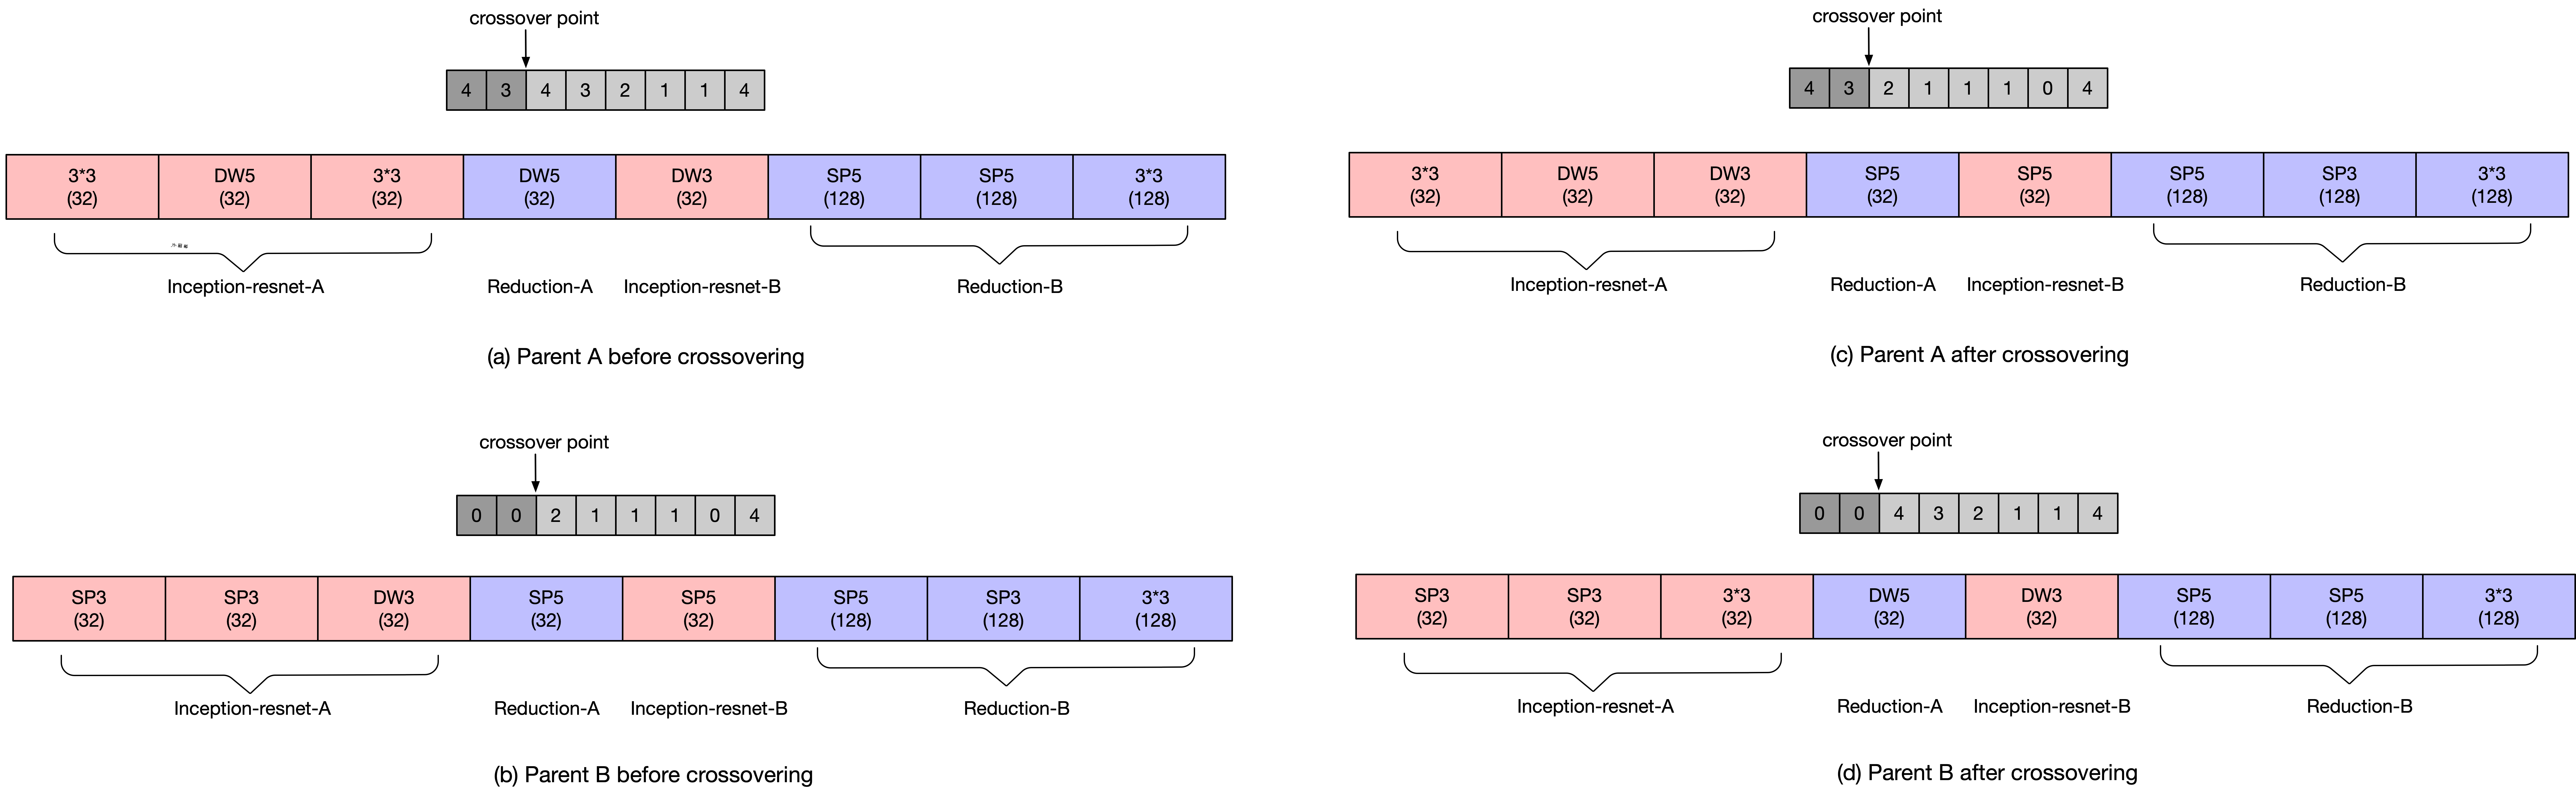
\includegraphics[width=7in]{cnn-cross}
\caption{CNN crossover operation.}
\label{fig_7}
\end{figure*}

\begin{figure*}[!t]
\centering
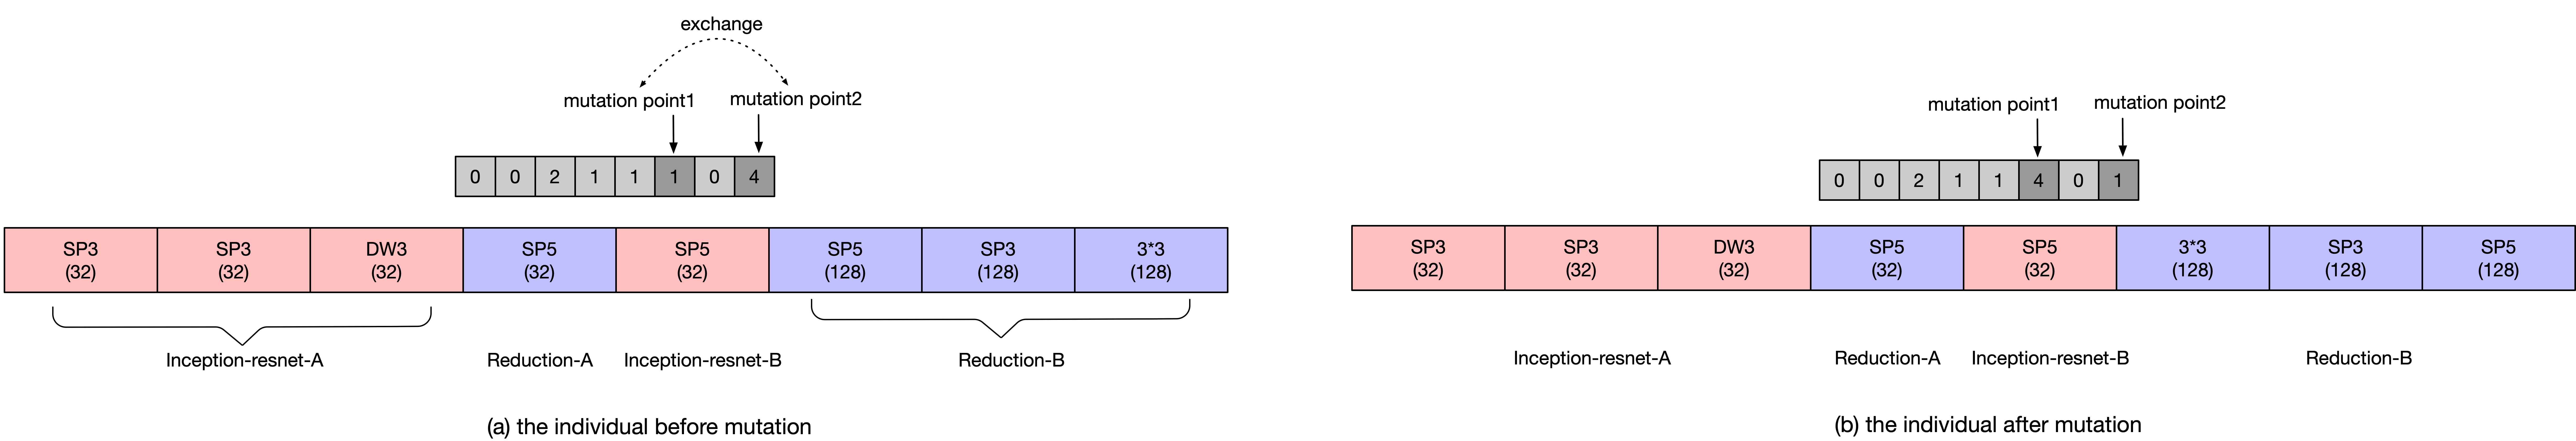
\includegraphics[width=7in]{cnn-mutation}
\caption{CNN mutation operation.}
\label{fig_8}
\end{figure*}

\section{EXPERIMENTAL RESULTS}\label{section_result}
\subsection{experiment setup and result}
Our network framework consists of GNN block and CNN block, so we need to convert the data into graph data and binary data according to the above method for adapting to our proposed architecture. Before the two network blocks, there is a reinforcement learning network, which is responsible for dynamically collecting the samples of the input detection model.
Our work is based on a publicly available datasets which is ATTACK \& DEFENSE CHALLENGE 2020 DATASET \cite{74} which is issues on IEEE-DATAPORT. the dataset contains two states of vehicle dynamic and stationary, and each part has two types of dataset files: intrusion and normal. In the intrusion file, several intrusion CAN messages are interspersed with normal message. Directly convert these labeled message into a format that can be input to the network for training and testing. Our task is to quickly and accurately identify the intrusion CAN messages from the dataset. Each dataset file has millions of CAN data frames, which can better extract various features in the message. We use the dynamic message part of the vehicle in the dataset, 80\% of the data are used for training and 20\% of the data are used for testing.

The CNN part trains 26 primary generations in advance, each individual trains 200 epochs, and takes the best accuracy as the adaptability index. Then, after 30 generations of crossover and mutation, the best 26 individuals are selected as the parents of the next generation, and so on. 30 generations of precision images are obtained as shown in figure \ref{fig_9}, It can be seen from the figure that with the evolution process, there are fewer and fewer individuals with low precision, and individuals with higher precision have evolved. After evolution the accuracy of every individual reached over 85\%. As shown in Table~\ref{table3}, although the accuracy of the end of evolution is almost the same as that of the early generation, in the last generation of evolution, the recognition accuracy of excellent individuals selected after training is 5\% higher than that of the first generation.

In the GNN part, first convert the data into graph data, and obtain the prediction results through graph coarsen, GCN, prediction layer, etc. The number of convolution layers and prediction layers of the graph network. The neurons of each prediction layer are optimized by EA. At the beginning, 100 primary generations were randomly generated, and 7 individuals at the Pareto front were selected from the primary generation as the parents of the next generation, evolving for 30 generations. As shown in figure \ref{fig_10} The complexity of 30 generations, flops, is x-axis, accuracy error, acc\_ error is the image of the y-axis. Red dots are used to mark the dots of the last  generations of individuals. Flops refers to the number of matrix operations in the process of network recognition. Divide by the number of matrix operations of hypernetwork, for converting the flops index into a range of 0 to 1. Acc\_ error refers to 1-acc, so the smaller the acc\_error, the higher the accuracy. It can be seen from the figure \ref{fig_10} that the last individual evolved to the position in the lower left corner of the figure, representing higher accuracy and lower complexity.

\begin{figure}[!t]
\centering
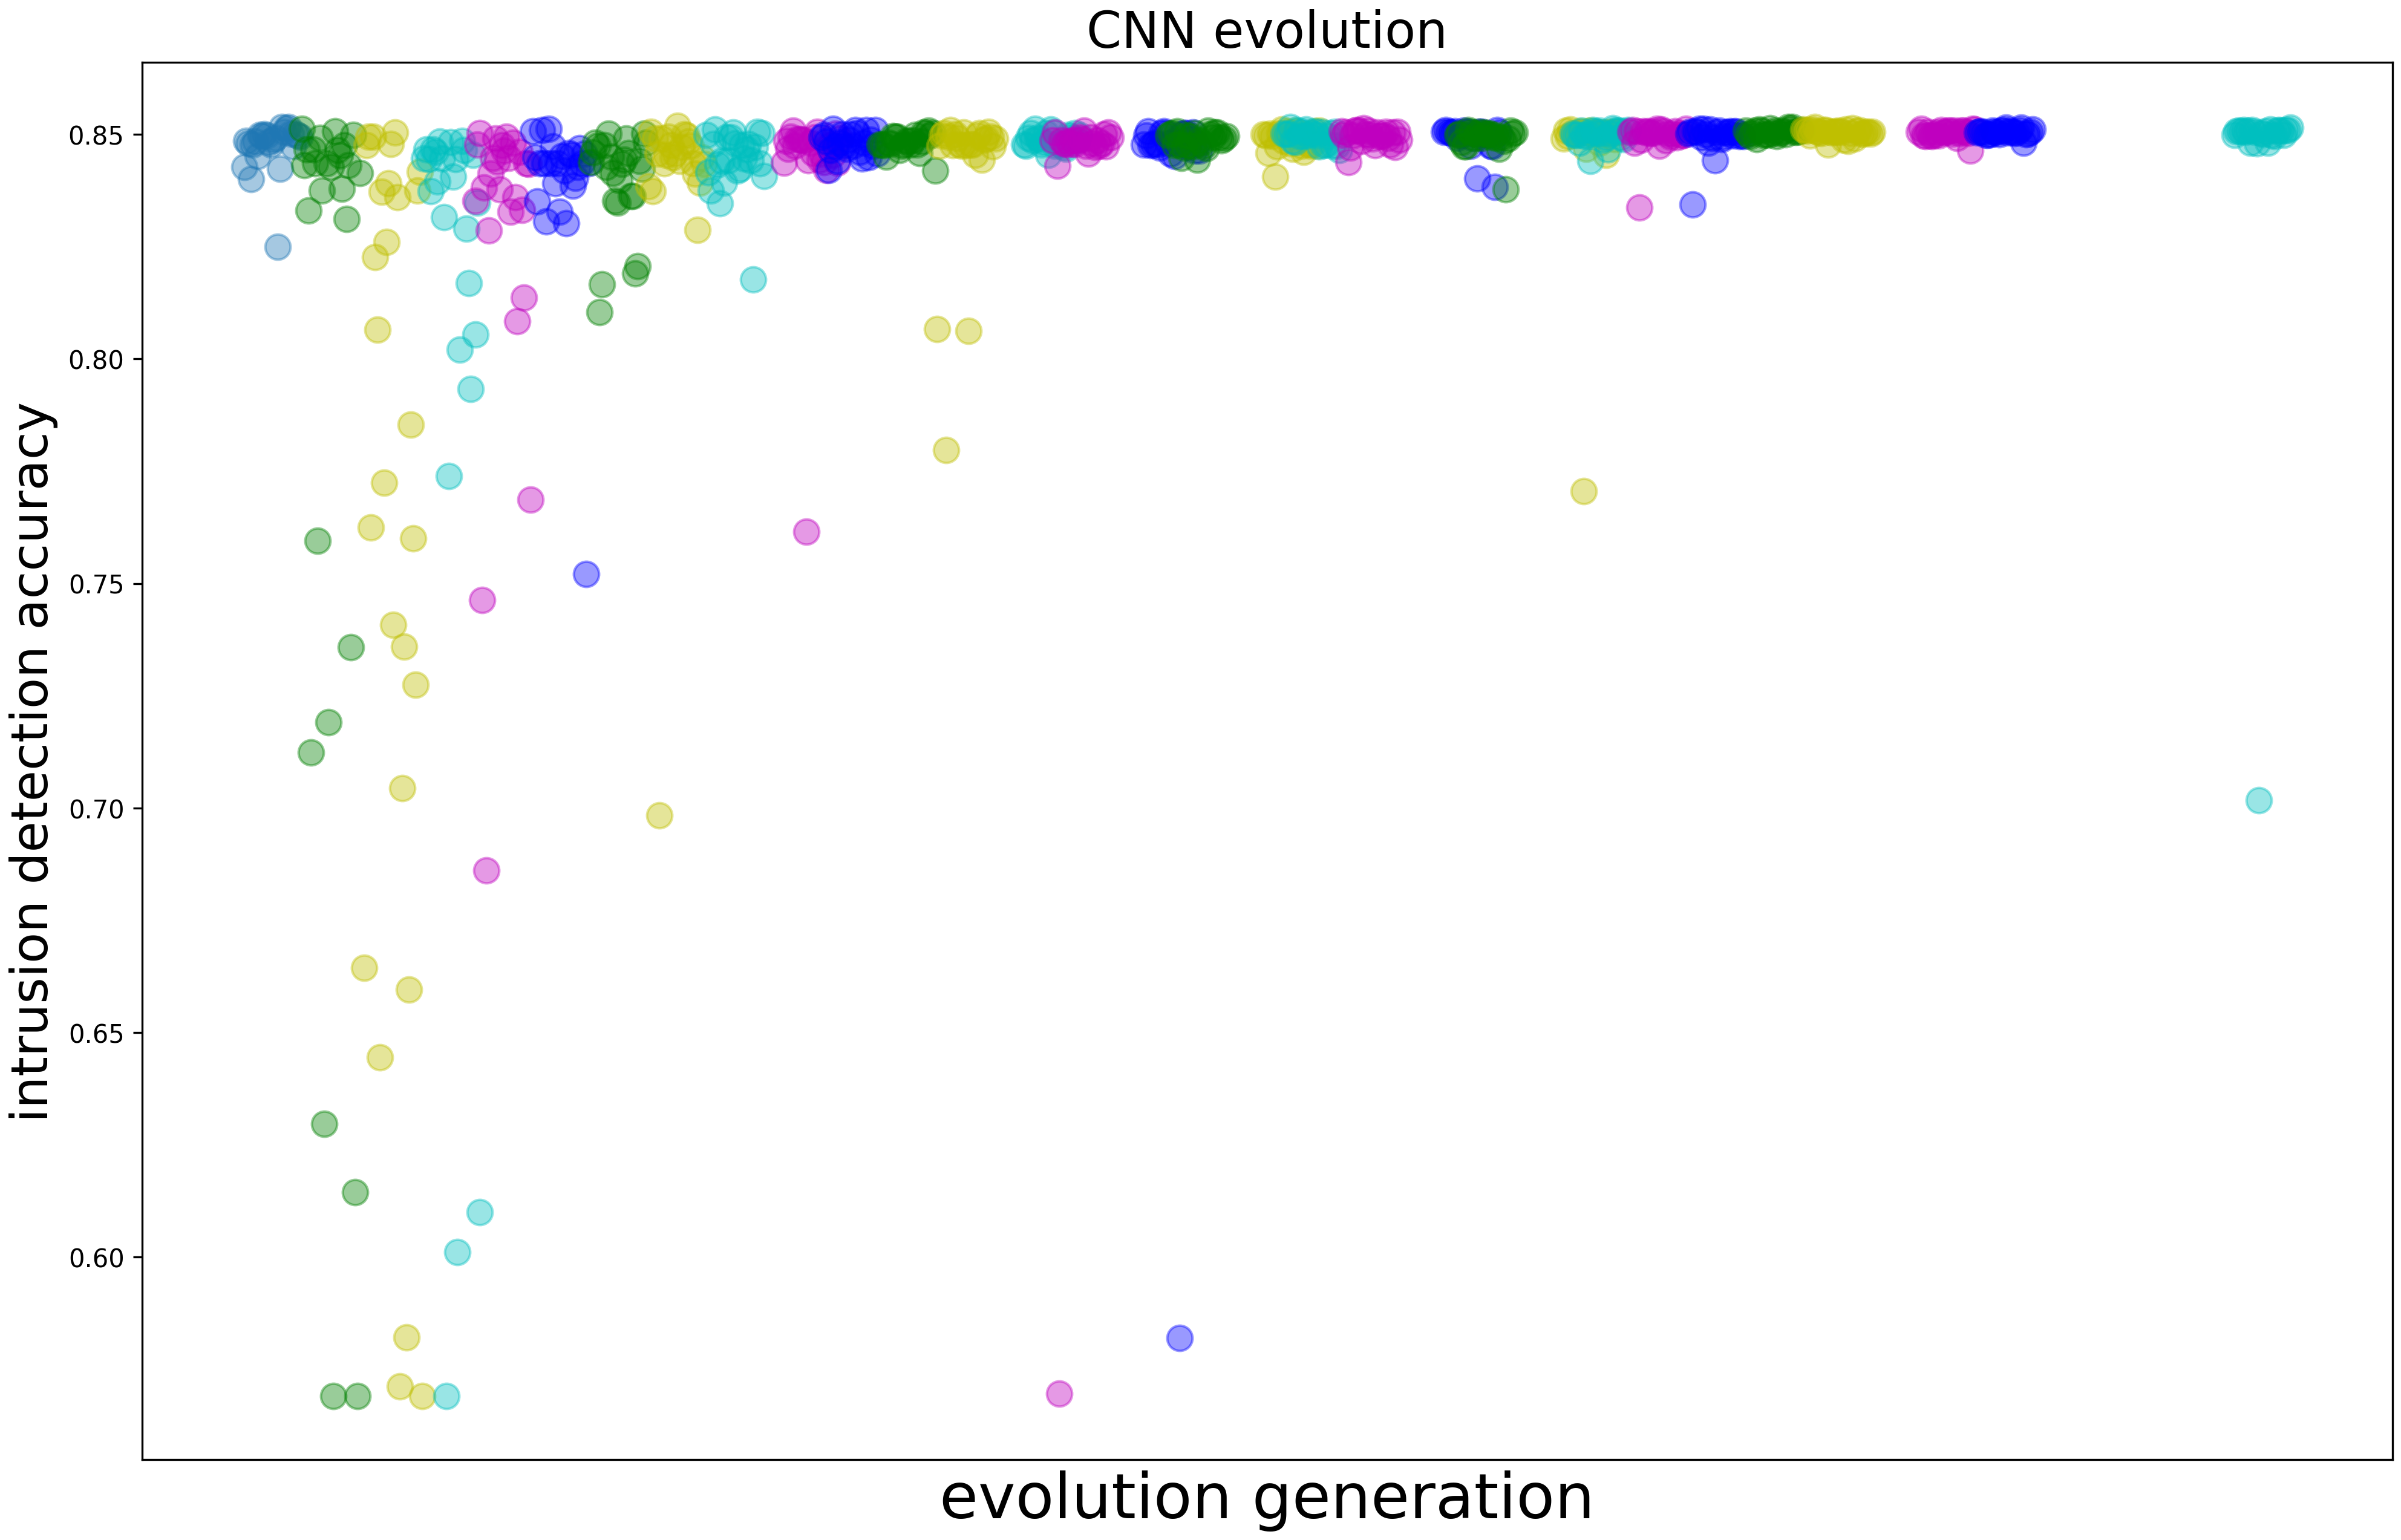
\includegraphics[width=3in]{cnn_evo}
\caption{CNN evolution result.}
\label{fig_9}
\end{figure}

\begin{table}[!t]
\caption{Individual comparison between early generation and post evolution\label{table3}}
\centering
\begin{tabular}{cccc}
\hline
stage & gene code & accuracy	 & flops\\
\hline
First Gen &  2,4,2,0,3,4,0,3 &  85.13\% &  2874.5M\\
After evolution without training & 4,4,4,2,3,0,2,3 & 85.15\% & 2628.7M\\
After evolution with training & 4,4,4,2,3,0,2,3 & 90.20\% & 2628.7M\\
\hline
\end{tabular}
\end{table}


\begin{figure}[!t]
\centering
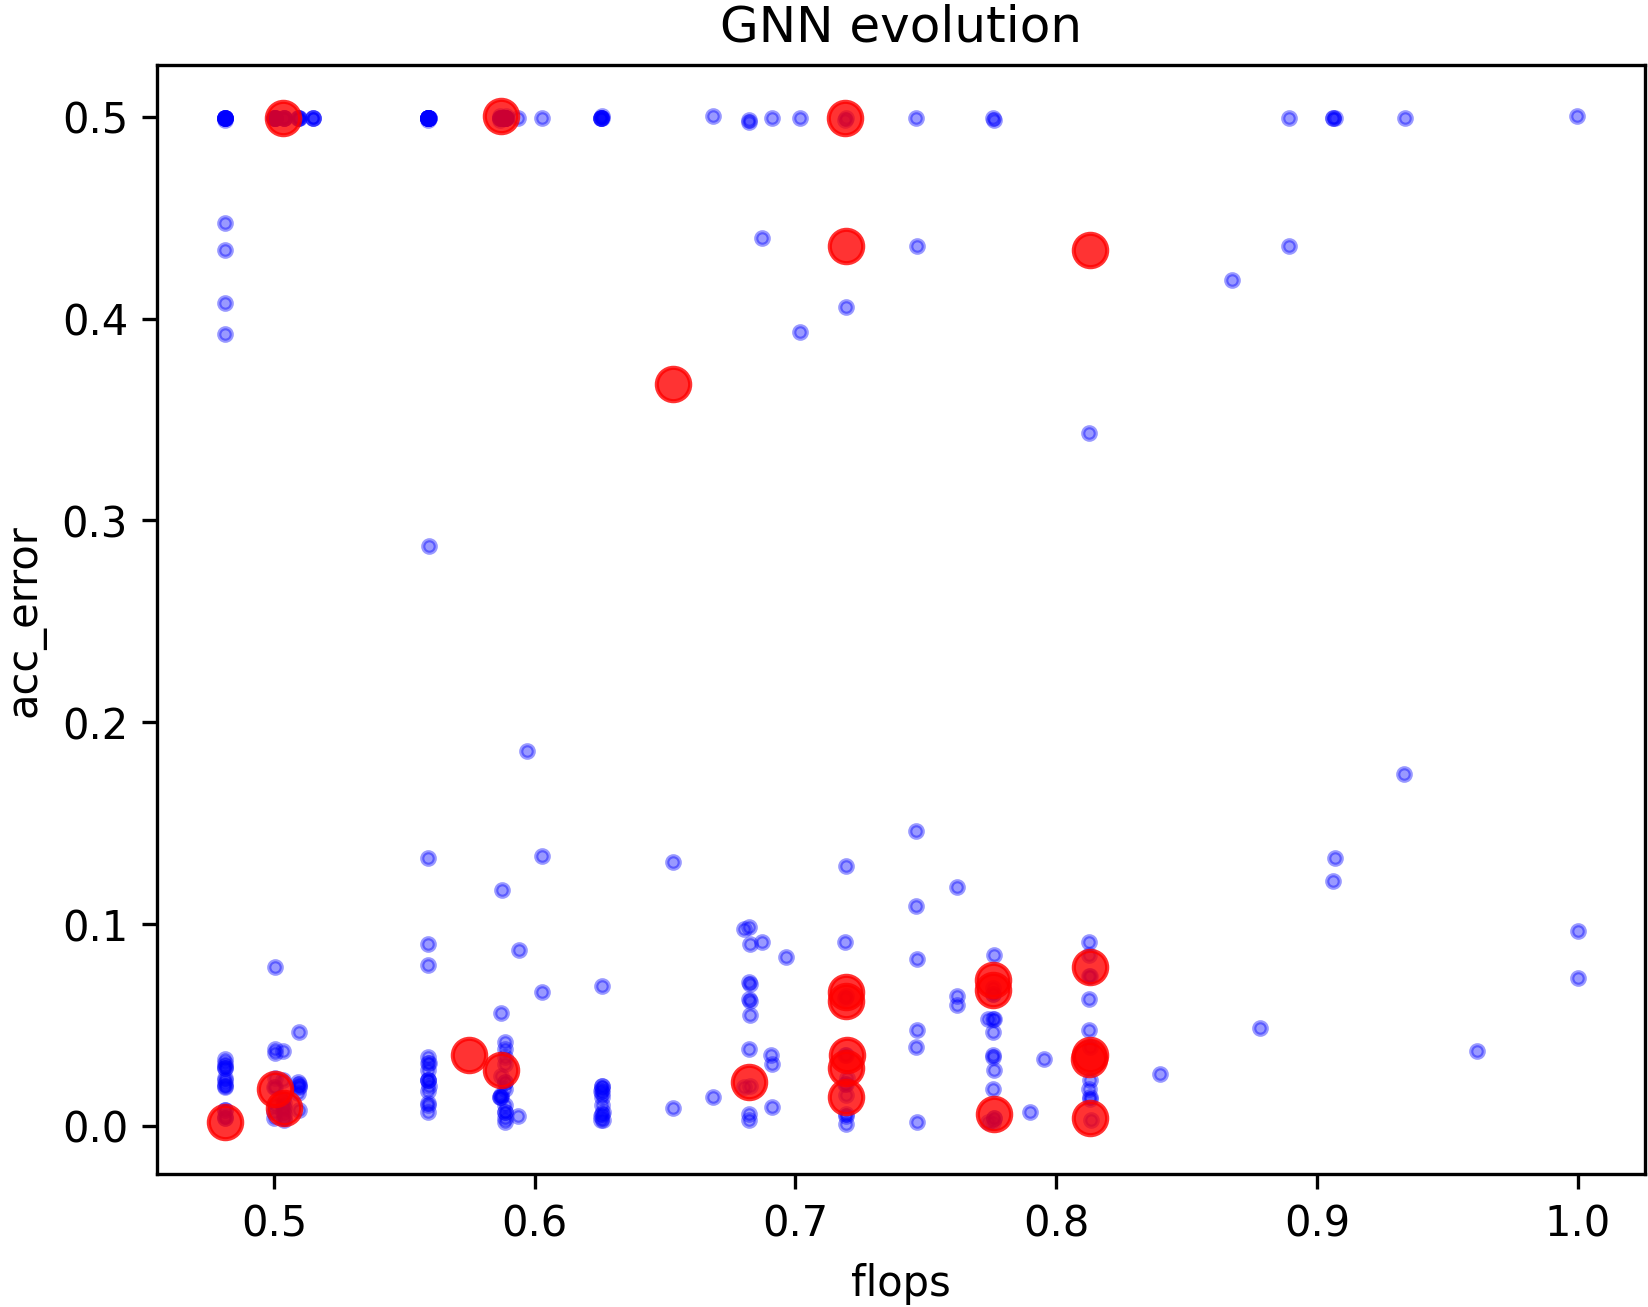
\includegraphics[width=3in]{gnn_evo}
\caption{GNN revolution result.}
\label{fig_10}
\end{figure}

We compared the impact of using the direction information of graph data on Intrusion Detection. The pooling matrix required for graph collapse classification is composed of eigenvectors of the Laplacian matrix of subgraphs. We also compare the impact of Laplacian matrix normalization on intrusion detection. It can be seen from the figure \ref{fig_11} that the result of using both graph data direction information and Laplace normalization is not the best. Removing the direction information of graph data will make the effect of intrusion detection better, so more use of graph data information will not necessarily improve the results of intrusion detection. Removing the Laplacian matrix normalization will also make the intrusion detection effect better, and also reduce the amount of calculation of data preprocessing. Therefore, it is reasonable to add the direction information of graph data and the normalization information of Laplace matrix into the search space. The final training results of the three networks can be seen from the Table~\ref{table4}.


\begin{figure}[!t]
\centering
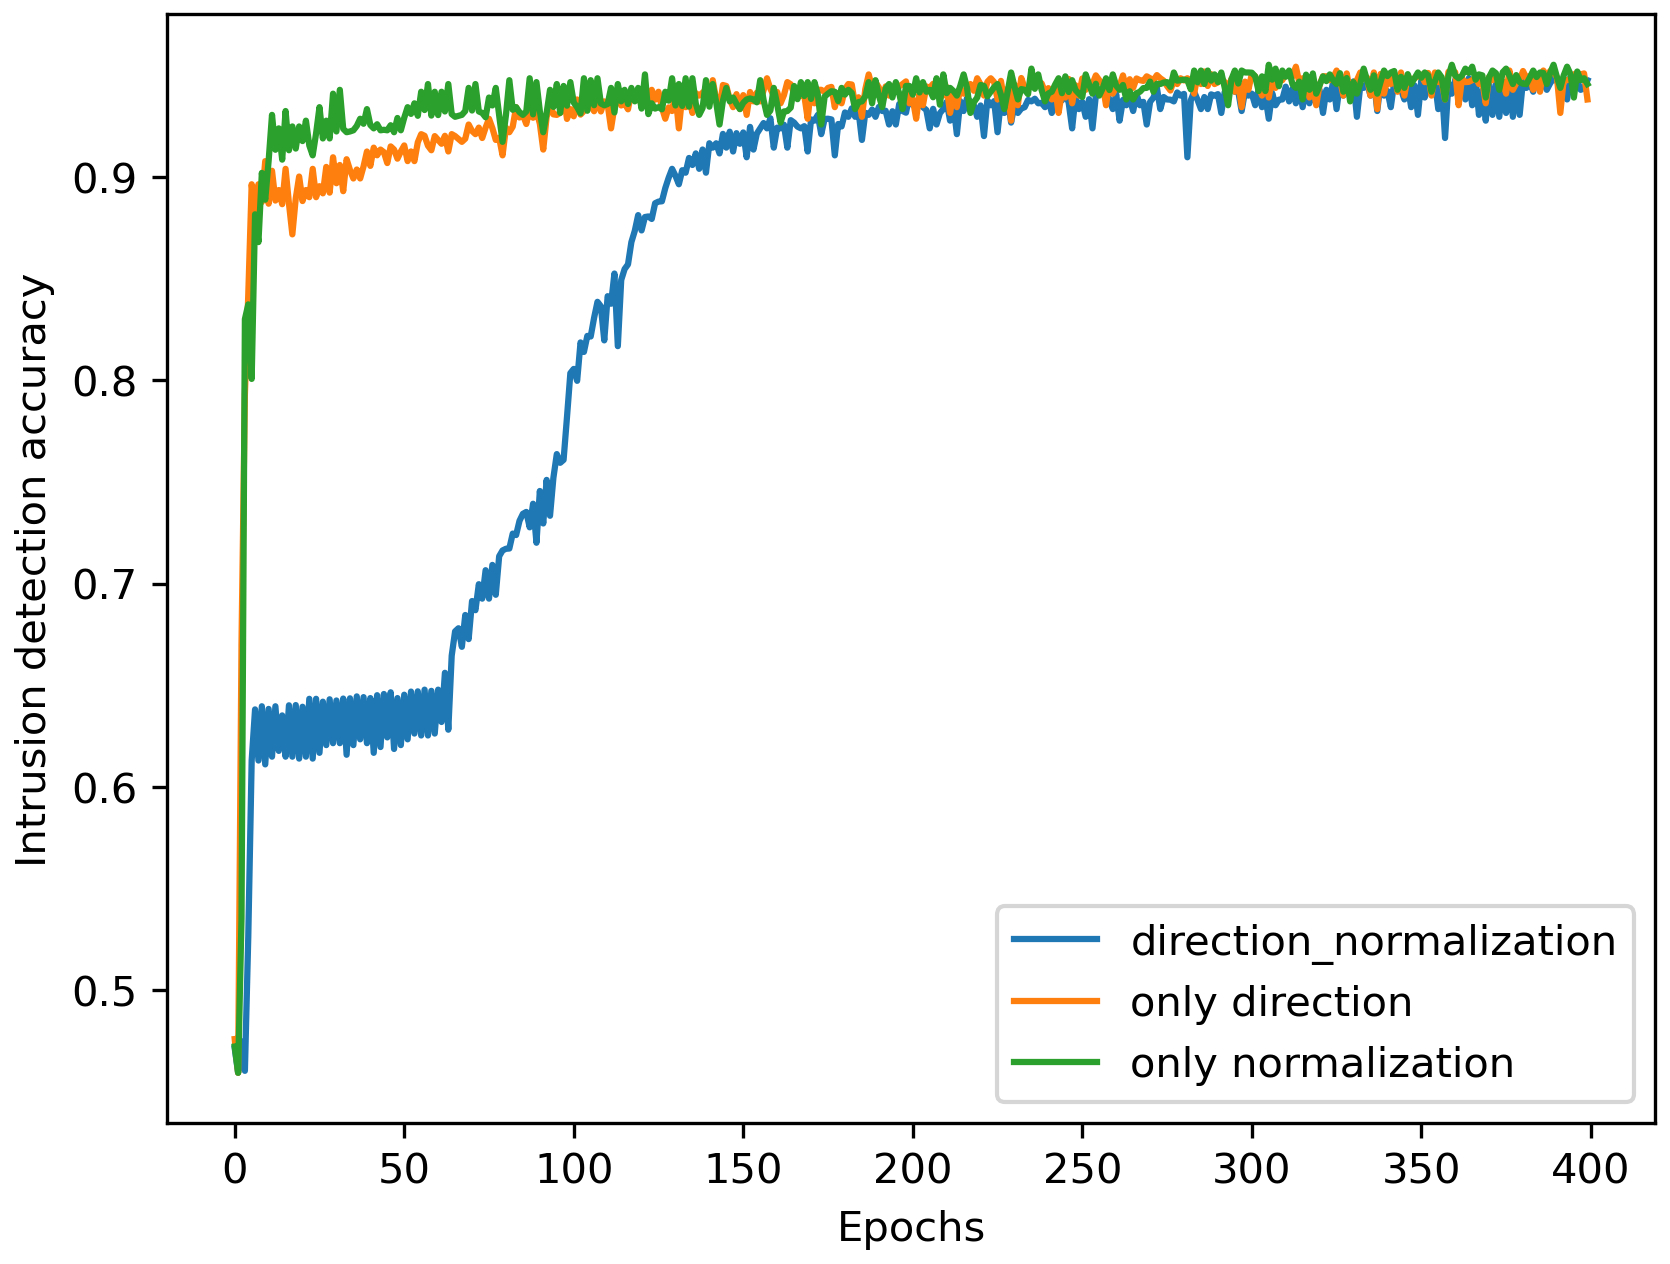
\includegraphics[width=3in]{di_nor_01}
\caption{The impact of graph data processing on Intrusion Detection.}
\label{fig_11}
\end{figure}

\begin{table}[!t]
\caption{comparison results of three GNNs\label{table4}}
\centering
\begin{tabular}{cc}
\hline
gene code & accuracy	\\
\hline
1100 0000 000 0021 0124 &  94.86\%\\
1000 0000 000 0021 0124 & 95.43\%\\
0100 0000 000 0021 0124 & 95.52\%\\
\hline
\end{tabular}
\end{table}

\subsection{compare with other deep learning method}
This experiment compares the experimental results of our method with LSTM, DNN, CNN and GNN. 
\cite{49} uses LSTM and Fully Connected Neural Network to extract the timing features of the data part of CAN. However, each CANID needs to train a complete neural network separately, so it is cumbersome. The loss function of the network is defined as the CrossEntropy loss of each bit corresponding to two adjacent frames of CAN messages. In the network verification stage, the maximum loss value of all bits is used as the basis for whether it is an intrusion message. Public dataset, Car\_Hacking\_Challenge\_Dataset\_rev20Mar2021\cite{74}, is used to training and verifying the neural network. Use the normal message part to train the LSTM network, and use the data mixed with abnormal message to test the network. We find that good results can be obtained after a small number of epochs. It is mentioned in the paper that some bits with low change frequency can be ignored by analyzing the data segment of CAN ID.
\cite{75} also uses the 64 bits data segment of CAN messages to directly input the bit stream to DNN network. The advantage of this network is that it is more efficient and can be directly input to the network without data processing. The specific architecture of the network is not pointed out in the paper. We adopt five layers of fully connection. The first layer has 64 neurons to receive 64 bits CAN messages bitstream, the second layer has 128 neurons, the third layer has 512 neurons, the fourth layer has 256 neurons, the fifth layer has 32 neurons, and the sixth layer outputs the second classification. Through the verification of public dataset, the accuracy is low, but the neural network is simple and does not need data preprocessing.
\cite{48} are the same with our network convolution part. I directly use our network framework. Using gene “44440444” can directly construct the same architecture as in the paper.  The dataset in \cite{48} is the data collected by the author himself. The classification accuracy of the public dataset does not reach the accuracy of the author's own experiment, which is lower than that of the convolution network we evolved by MOEA. Our algorithm combines the two advantages of the spatial feature extraction of CNN and the logical feature of GNN, compares the difference of two-dimensional variables output by the two networks when outputting the results, and takes the network result with large difference as the final result, which is the result of taking a network that is more confident in the intrusion detection. Using this method, the two forms of networks can complement each other. As shown in the Table~\ref{table5}, it is the comparison result of these network architectures. It can be seen that our network can achieve higher recognition accuracy, which is very important for network security. GNN module is also a part of the neural network architecture proposed by us. From the results, it can be seen that the accuracy of a single GNN network is lower than that of the combination of two networks.

\begin{table}[!t]
\caption{CNN search space\label{table5}}
\centering
\begin{tabular}{cccc}
\hline
deep learning method & accuracy & flops\\
\hline
LSTM\cite{49} & 97.02\% & 3.6M\\
DNN\cite{75} & 95.36\% & 6.8M\\
GNN & 96.43\% & 54.3M\\
CNN\cite{48} & 85.06\% & 2628.7M\\
our method without RL & 95.17\% & 2673.1M\\
our method with RL & \textbf{99.87}\% & 2673.1M\\
\hline
\end{tabular}
\end{table}

\section{CONCLUSION AND FUTURE WORK}\label{section_conclusion}
We use multiple network composition to ensure the accuracy of intrusion detection and minimize the complexity of the network. As far as we know, GNN is used for CAN intrusion detection for the first time in this work, and only GNN detection results can reach more than 95\%. At the same time, we combine the dual advantages of graph network and convolution network. Through the output results of the two networks, the detection results of the two networks are complementary. At the same time, the logical and spatial characteristics of CAN are used. There are still some deficiencies in this work. Although it can achieve pretty good recognition accuracy, compared with previous work, the complexity of our network is higher. Our future work can further apply evolutionary algorithm to simplify the architecture of the network more carefully. The combination model of graph network and LSTM network can be considered to reduce model’s complexity and obtain better result. This work is to search the architecture of CNN and GNN respectively. It can be considered to search the overall architecture of RL, CNN and GNN at the same time, so as to improve the detection accuracy and reduce the complexity. Increasing the number of the objective function of the MOEA, such as false positive rate and true positive rate, to obtain better intrusion detection model.

%\section*{Acknowledgments}
%This should be a simple paragraph before the References to thank those individuals and institutions who have supported your work on this article.



%{\appendix[Proof of the Zonklar Equations]
%Use $\backslash${\tt{appendix}} if you have a single appendix:
%Do not use $\backslash${\tt{section}} anymore after $\backslash${\tt{appendix}}, only $\backslash${\tt{section*}}.
%If you have multiple appendixes use $\backslash${\tt{appendices}} then use $\backslash${\tt{section}} to start each appendix.
%You must declare a $\backslash${\tt{section}} before using any $\backslash${\tt{subsection}} or using $\backslash${\tt{label}} ($\backslash${\tt{appendices}} by itself
% starts a section numbered zero.)}



%{\appendices
%\section*{Proof of the First Zonklar Equation}
%Appendix one text goes here.
% You can choose not to have a title for an appendix if you want by leaving the argument blank
%\section*{Proof of the Second Zonklar Equation}
%Appendix two text goes here.}



%\section{References Section}
%You can use a bibliography generated by BibTeX as a .bbl file.
% BibTeX documentation can be easily obtained at:
% http://mirror.ctan.org/biblio/bibtex/contrib/doc/
% The IEEEtran BibTeX style support page is:
% http://www.michaelshell.org/tex/ieeetran/bibtex/
 
 % argument is your BibTeX string definitions and bibliography database(s)
%\bibliography{IEEEabrv,../bib/paper}
%
%\section{Simple References}
%You can manually copy in the resultant .bbl file and set second argument of $\backslash${\tt{begin}} to the number of references
% (used to reserve space for the reference number labels box).

\bibliography{paper}
\bibliographystyle{IEEEtran}


%\newpage
%
%\section{Biography Section}
%If you have an EPS/PDF photo (graphicx package needed), extra braces are
% needed around the contents of the optional argument to biography to prevent
% the LaTeX parser from getting confused when it sees the complicated
% $\backslash${\tt{includegraphics}} command within an optional argument. (You can create
% your own custom macro containing the $\backslash${\tt{includegraphics}} command to make things
% simpler here.)
% 
%\vspace{11pt}
%
%%\bf{If you include a photo:}\vspace{-33pt}
%%\begin{IEEEbiography}[{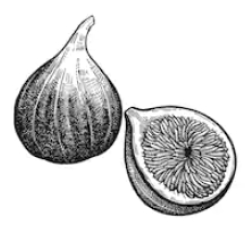
\includegraphics[width=1in,height=1.25in,clip,keepaspectratio]{fig1}}]{Michael Shell}
%%Use $\backslash${\tt{begin\{IEEEbiography\}}} and then for the 1st argument use $\backslash${\tt{includegraphics}} to declare and link the author photo.
%%Use the author name as the 3rd argument followed by the biography text.
%%\end{IEEEbiography}
%
%\vspace{11pt}
%
%\bf{If you will not include a photo:}\vspace{-33pt}
%\begin{IEEEbiographynophoto}{John Doe}
%Use $\backslash${\tt{begin\{IEEEbiographynophoto\}}} and the author name as the argument followed by the biography text.
%\end{IEEEbiographynophoto}
%
%
%
%
%\vfill

\end{document}